\documentclass[handout]{beamer}
%==============================================================
% Common Beamer Preamble for Course Lectures: Training and Scaling Language Models
%==============================================================

\usepackage[utf8]{inputenc}
\usepackage[T1]{fontenc}
\usepackage{hyperref}
\usepackage{amsmath,amssymb,xcolor,multicol,booktabs,colortbl}
\usepackage{graphicx,listings}
\renewcommand{\figurename}{Figure.}
\renewcommand{\tablename}{Table.}

% ---- TikZ Libraries ----
\usepackage{tikz}
\usetikzlibrary{positioning,arrows.meta,shapes.geometric,calc,fit,backgrounds,decorations.pathreplacing}

% ---- Presentation defaults ----
\setbeamertemplate{navigation symbols}{}
\setbeamersize{text margin left=0.55cm,text margin right=0.55cm}
\setbeamerfont{title}{size=\LARGE,series=\bfseries}
\setbeamerfont{subtitle}{size=\large}

% ---- FontAwesome fallback ----
\IfFileExists{fontawesome5.sty}{%
  \usepackage{fontawesome5}%
}{%
  \providecommand{\faMicrochip}{}%
  \providecommand{\faComments}{}%
  \providecommand{\faTools}{}%
  \providecommand{\faCheckCircle}{}%
  \providecommand{\faExclamationTriangle}{}%
  \providecommand{\faImage}{}%
  \providecommand{\faRobot}{}%
  \providecommand{\faTerminal}{}%
  \providecommand{\faBook}{}%
  \providecommand{\faRedo}{}%
  \providecommand{\faLayerGroup}{}%
  \providecommand{\faCogs}{}%
  \providecommand{\faDatabase}{}%
  \providecommand{\faHdd}{}%
  \providecommand{\faNetworkWired}{}%
}

% ---- Theme Style and Semantic Colors ----
%==============================================================
% Centralized Semantic Color Definitions for LLMs Presentation
%==============================================================

% ---- Base Template / Theme Colors (Aligned with Palette B) ----
\definecolor{themenavy}{RGB}{22,70,102}       % Palette B primary cerulean: #164666
\definecolor{themeblue}{RGB}{22,70,102}       % Primary alias
\definecolor{primarylight}{RGB}{34,92,132}    % Primary light: #225c84
\definecolor{themeteal}{RGB}{0,159,176}       % Accent cyan-teal: #009fb0
\colorlet{main_color}{themenavy}
\colorlet{accent}{themeteal}

\definecolor{accentdark}{RGB}{0,108,120}      % Deep cyan-teal for contrast text
\definecolor{accentlight}{RGB}{56,178,214}    % Slate accent cyan: #38b2d6
\definecolor{leafred}{RGB}{197,93,61}         % Terracotta red for branches/leaves

% ---- Website Panel & Border Neutrals ----
\definecolor{panelbg}{RGB}{237,245,249}       % Course-panel: #edf5f9
\definecolor{panelborder}{RGB}{204,226,238}   % Course-border: #cce2ee

% ---- Code listing style (syntax highlights) ----
\definecolor{deepblue}{RGB}{22,70,102}
\definecolor{deepred}{rgb}{0.6,0,0}
\definecolor{deepgreen}{RGB}{0,135,150}
\definecolor{halfgray}{gray}{0.55}

% ---- Semantic Theme Navy / Cerulean Shades ----
\colorlet{themebluebg}{panelbg}               % Panel #edf5f9
\colorlet{themebluecard}{main_color!8}        % Mild card background fills
\colorlet{themeblueborder}{panelborder}       % Border #cce2ee
\colorlet{themebluemid}{themeteal!60}         % Accent mid-contrast
\colorlet{themebluedraw}{main_color!80}       % Strong outline draws/strokes

% ---- Semantic Secondary Accent Teal Shades ----
\colorlet{accentdarkbg}{themeteal!10}        % Light secondary background fills
\colorlet{accentdarkdraw}{themeteal}         % Secondary outlines/strokes/text/axes

% ---- Functional Colors: Success Green ----
\definecolor{successgreen}{RGB}{55,145,55}
\colorlet{successbg}{successgreen!8}
\colorlet{successdraw}{successgreen!75}

% ---- Functional Colors: Alert Red ----
\definecolor{alertred}{RGB}{197,55,55}
\colorlet{alertbg}{alertred!8}
\colorlet{alertdraw}{alertred!75}

% ---- Functional Colors: Warning Orange ----
\definecolor{warningorange}{RGB}{220,110,30}
\colorlet{warningbg}{warningorange!10}
\colorlet{warningdraw}{warningorange!80}

% ---- Terracotta Red Shades ----
\colorlet{leafredbg}{leafred!12}
\colorlet{leafreddraw}{leafred!80}

% ---- Accent Violet (SWE-bench / observe phases) ----
\definecolor{accentviolet}{RGB}{120,70,180}
\colorlet{accentvioletbg}{accentviolet!10}
\colorlet{accentvioletdraw}{accentviolet!80}

% ---- Post-Training Axis Blue ----
\definecolor{posttrainingblue}{RGB}{40,90,165}
\colorlet{posttrainingbg}{posttrainingblue!8}
\colorlet{posttrainingdraw}{posttrainingblue!75}

% ---- Harness Component Action Green ----
\definecolor{actiongreen}{RGB}{55,145,55}
\colorlet{actiongreenbg}{actiongreen!10}
\colorlet{actiongreendraw}{actiongreen!65}

% ---- Harness Component Persist Olive ----
\definecolor{persistolive}{RGB}{120,135,40}
\colorlet{persistolivebg}{persistolive!12}
\colorlet{persistolivedraw}{persistolive!70}

% ---- Harness Component Observe Violet ----
\colorlet{observevioletbg}{accentvioletbg}
\colorlet{observevioletdraw}{accentvioletdraw}

% ---- Neutrals (Grays/Blacks) ----
\colorlet{neutralbg}{black!4}             % Very light background fills
\colorlet{neutrallight}{black!30}         % Border frames/ticks/dividers
\colorlet{neutraldark}{black!75}          % Main body text/code listing text

% ---- Beamer Block Color Overrides (Premium Terracotta Theme) ----
\setbeamercolor{block title alert}{bg=leafreddraw,fg=white}
\setbeamercolor{block body alert}{bg=leafredbg}
\setbeamercolor{alerted text}{fg=leafreddraw}

\usepackage{../common/style}
\graphicspath{{../common/figs/}{figs/}}

% ---- Code Listing Config ----
\lstset{
  basicstyle=\ttfamily\footnotesize,
  keywordstyle=\bfseries\color{deepblue},
  emphstyle=\ttfamily\color{deepred},
  stringstyle=\color{deepgreen},
  commentstyle=\color{halfgray}\itshape,
  numbers=left, numberstyle=\tiny\color{halfgray},
  backgroundcolor=\color{codebg},
  frame=l, framerule=1.5pt, rulecolor=\color{themeteal},
  xleftmargin=10pt, framexleftmargin=4pt, numbersep=6pt,
  showstringspaces=false, breaklines=true,
  aboveskip=4pt, belowskip=4pt
}

% ---- Image Placeholder Utility ----
\newcommand{\slideimage}[2][3.8cm]{%
  \begin{center}
    \begin{tikzpicture}
      \node[draw=main_color, dashed, very thick, rounded corners,
        fill=themebluebg, minimum width=0.88\linewidth, minimum height=#1,
      text width=0.80\linewidth, align=center, font=\itshape, text=accentdark]
      {\textbf{[ FIGURE / DIAGRAM ]}\\[6pt] #2};
    \end{tikzpicture}
  \end{center}
}

% ---- Concept Highlight Card Utility ----
\newcommand{\conceptcard}[3]{%
  \begin{coursebox}{#1}{#2}#3\end{coursebox}%
}

% ---- Reusable teaching-slide components ----
\newcommand{\learninggoals}[4]{%
  \begin{frame}{What should be clear by the end?}
    \begin{enumerate}
        \setlength{\itemsep}{7pt}
      \item #1
      \item #2
      \item #3
      \item #4
    \end{enumerate}
  \end{frame}
}

\newcommand{\checkpoint}[2]{%
  \begin{frame}{Checkpoint: #1}
    \begin{block}{Think, then compare}
      #2
    \end{block}
  \end{frame}
}

\newcommand{\takeaways}[4]{%
  \begin{frame}{The durable ideas}
    \begin{enumerate}
        \setlength{\itemsep}{8pt}
      \item #1
      \item #2
      \item #3
      \item #4
    \end{enumerate}
  \end{frame}
}

\newcommand{\smallsource}[1]{%
  \vfill\hfill{\tiny\color{neutraldark}Source: #1}
}

% ---- Logo on content frames ----
\newif\ifplacelogo
\placelogotrue
\logo{\ifplacelogo
  \raisebox{-0.3ex}{
\includegraphics[height=0.4cm]{IMT_Atlantique_logo.png}}%
\fi}

\makeatletter
\define@key{beamerframe}{nologo}[true]{%
  \placelogofalse
}
\makeatother

% Fix Beamer bold font warning: substitute undefined T1/cmss/b/n with T1/cmss/bx/n
\DeclareFontShape{T1}{cmss}{b}{n}{<->ssub * cmss/bx/n}{}

% Default Author & Institute metadata
\author[Jonathan Lys]{Jonathan Lys}
\institute[IMT Atlantique]{IMT Atlantique}

% ---- Front Page / Title Slide Macro ----
% Displays Title + IMT Atlantique logo and Brain logo
\newcommand{\makelecturetitle}[1][Training and Scaling Language Models: From First Principles to Efficient Serving]{%
  \placelogofalse
  {
    \setbeamertemplate{footline}{}
    \settitletagline{#1}
    \settitlelogos{%
      \raisebox{-0.5\height}{
\includegraphics[height=1.15cm]{IMT_Atlantique_logo.png}}%
      \hspace{1.2em}%
      \raisebox{-0.5\height}{\includegraphics[height=1.15cm]{brain.pdf}}}
    \begin{frame}[plain]
      \titlepage
    \end{frame}
  }
  \placelogotrue
}

% Section TOC Frame
\AtBeginSection[]{\coursesectiondivider}


\title[TLM -- Session 03]{Session 3: BPE and the Data Pipeline\\[4pt]
\normalsize\itshape From Raw Documents to Verified Token Batches}
\date{\today}

\begin{document}
\makelecturetitle

\begin{frame}{Lecture map}
  \tableofcontents
  \vfill
  \begin{block}{Guiding question}
    How do we turn irregular text into dense, reproducible GPU input without changing the learning task?
  \end{block}
\end{frame}

\learninggoals
  {Explain byte-level BPE as a learned compression code.}
  {Reason about vocabulary size, sequence length, and parameter cost together.}
  {Pack documents while keeping boundaries explicit.}
  {Verify binary storage, sampling, and the next-token shift.}

\section{A tokenizer is a model design choice}

\begin{frame}{Granularity moves cost between vocabulary and sequence}
  \small
  \begin{tabular}{llll}
    \toprule
    Unit & Vocabulary & Sequence & Main cost \\
    \midrule
    bytes & 256 & very long & attention and context \\
    words & millions & short & embeddings and unknowns \\
    subwords & tunable & moderate & learned merge system \\
    \bottomrule
  \end{tabular}
  \vfill
  \begin{block}{Why byte-level BPE?}
    Every UTF-8 string decomposes into 256 byte values, so the base system has no unknown text. Frequent byte sequences can then become single tokens.
  \end{block}
  \begin{alertblock}{System consequence}
    Tokenization changes sequence length, attention work, KV-cache size, multilingual efficiency, and the number of embedding parameters.
  \end{alertblock}
\end{frame}

\begin{frame}{BPE learns a greedy compression hierarchy}
  \begin{enumerate}
    \setlength{\itemsep}{6pt}
    \item Start from byte IDs and reserved special tokens.
    \item Count adjacent token pairs in the training corpus.
    \item Merge the most frequent pair into one new token.
    \item Repeat until the vocabulary reaches its target size.
  \end{enumerate}
  \[
    (p_0,p_1)\mapsto v_{\text{new}},
    \qquad
    \operatorname{repr}(v_{\text{new}})=
    \operatorname{repr}(p_0)\Vert\operatorname{repr}(p_1)
  \]
  \begin{block}{Encoding new text}
    Apply learned merges by rank. Earlier learned pairs win when several merges are possible.
  \end{block}
  \smallsource{Gage, Sennrich et al., GPT-2, and minBPE}
\end{frame}

\begin{frame}{A hand-worked merge exposes the algorithm}
  Corpus: \texttt{low low lower}
  \vspace{4pt}
  \begin{center}
  \begin{tabular}{lll}
    \toprule
    Round & frequent pair & stream fragment \\
    \midrule
    0 & -- & \texttt{l o w | l o w | l o w e r} \\
    1 & \texttt{l o} & \texttt{lo w | lo w | lo w e r} \\
    2 & \texttt{lo w} & \texttt{low | low | low e r} \\
    \bottomrule
  \end{tabular}
  \end{center}
  \begin{alertblock}{What the table hides}
    Real byte-level training also defines deterministic tie-breaking, special-token policy, and merge boundaries. These are part of the tokenizer artifact.
  \end{alertblock}
\end{frame}

\begin{frame}{Pre-tokenization prevents pathological merges}
  \begin{columns}[c]
    \begin{column}{0.48\linewidth}
      \begin{alertblock}{Naive byte stream}
        Frequent punctuation and whitespace can merge across unrelated words or document structure.
      \end{alertblock}
    \end{column}
    \begin{column}{0.48\linewidth}
      \begin{block}{Regex chunks}
        Letters, numbers, punctuation, contractions, and whitespace form separate regions. BPE merges stay inside each region.
      \end{block}
    \end{column}
  \end{columns}
  \vfill
  \centering
  \texttt{" the"} and \texttt{"the"} may become different learned tokens because leading-space behavior carries information.
\end{frame}

\begin{frame}{Vocabulary size has two opposing effects}
  \begin{columns}[c]
    \begin{column}{0.52\linewidth}
      \begin{block}{Larger vocabulary}
        fewer tokens per document\\lower attention and decode length\\better compression for frequent patterns
      \end{block}
    \end{column}
    \begin{column}{0.44\linewidth}
      \begin{alertblock}{But also}
        larger embedding and output matrices\\rarer tail tokens\\more expensive vocabulary softmax
      \end{alertblock}
    \end{column}
  \end{columns}
  \[
    \text{embedding parameters}=Vd
    \qquad
    \text{compression}=\frac{\text{UTF-8 bytes}}{\text{tokens}}
  \]
  \centering Weight tying avoids paying $Vd$ twice.
\end{frame}

\checkpoint{tokenizer choice}
  {A new tokenizer shortens a representative corpus by 20\% but adds 300 million embedding parameters. Which training and serving measurements would decide whether this is a good trade?}

\section{Packing documents into examples}

\begin{frame}{Padding turns document length variance into wasted FLOPs}
  \begin{center}
    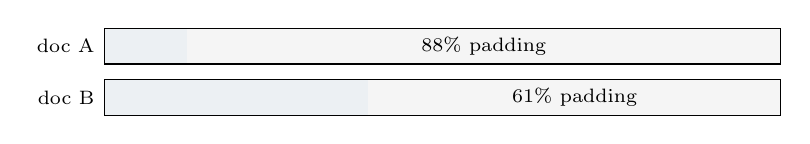
\begin{tikzpicture}[x=.0042cm,y=.65cm,every node/.style={font=\scriptsize}]
      \fill[themebluecard] (0,2) rectangle (250,2.7);
      \fill[neutralbg] (250,2) rectangle (2048,2.7);
      \draw (0,2) rectangle (2048,2.7);
      \node[left] at (0,2.35) {doc A};
      \node at (1149,2.35) {88\% padding};
      \fill[themebluecard] (0,1) rectangle (800,1.7);
      \fill[neutralbg] (800,1) rectangle (2048,1.7);
      \draw (0,1) rectangle (2048,1.7);
      \node[left] at (0,1.35) {doc B};
      \node at (1424,1.35) {61\% padding};
    \end{tikzpicture}
  \end{center}
  \begin{block}{Dense packing}
    Concatenate documents with an explicit end-of-text token, then slice fixed-length training windows from the resulting token stream.
  \end{block}
\end{frame}

\begin{frame}{Packing improves utilization but changes attention structure}
  \begin{columns}[c]
    \begin{column}{0.56\linewidth}
      \texttt{[doc A][EOT][doc B][EOT][doc C]}
      \vspace{8pt}
      \begin{itemize}
        \setlength{\itemsep}{7pt}
        \item Every position contributes to the loss.
        \item Windows can cross a document boundary.
        \item Standard causal attention lets doc B see doc A.
      \end{itemize}
    \end{column}
    \begin{column}{0.40\linewidth}
      \begin{block}{Two valid policies}
        Accept cross-document context and record it.\\[6pt]
        Or use block-diagonal causal masks with document offsets.
      \end{block}
    \end{column}
  \end{columns}
  \begin{alertblock}{Invariant}
    Train and validation splits must happen at the document level before packing.
  \end{alertblock}
\end{frame}

\begin{frame}{The end-of-text token has two roles}
  \begin{enumerate}
    \setlength{\itemsep}{9pt}
    \item It preserves a recoverable boundary in a contiguous stream.
    \item It teaches the model that one document ended and another may begin.
  \end{enumerate}
  \begin{alertblock}{Special-token policy}
    Reserve its ID before training merges. Prevent ordinary text from being confused with the special marker. Test round-trip behavior explicitly.
  \end{alertblock}
\end{frame}

\section{Storage and correctness}

\begin{frame}{Binary shards remove tokenization from the hot path}
  \begin{columns}[c]
    \begin{column}{0.55\linewidth}
      \begin{itemize}
        \setlength{\itemsep}{8pt}
        \item Pre-tokenize once and store integer IDs contiguously.
        \item Use \texttt{uint16} only when every ID fits below $65{,}536$.
        \item Open shards with memory mapping and let the OS page cache serve workers.
      \end{itemize}
    \end{column}
    \begin{column}{0.41\linewidth}
      \begin{block}{Storage estimate}
        $10^9$ tokens at 2 bytes each occupy 2.0 GB before metadata.
      \end{block}
      \begin{alertblock}{Schema contract}
        Record dtype, tokenizer hash, token count, and document-boundary convention beside each shard.
      \end{alertblock}
    \end{column}
  \end{columns}
\end{frame}

\begin{frame}{One contiguous slice creates inputs and targets}
  Sample $T+1$ tokens beginning at offset $i$:
  \[
    x = s[i:i+T]
    \qquad
    y = s[i+1:i+T+1]
  \]
  \begin{center}
    \begin{tabular}{c|ccccc}
      & 0 & 1 & 2 & $\cdots$ & $T-1$ \\
      \hline
      $x$ & $s_i$ & $s_{i+1}$ & $s_{i+2}$ & $\cdots$ & $s_{i+T-1}$ \\
      $y$ & $s_{i+1}$ & $s_{i+2}$ & $s_{i+3}$ & $\cdots$ & $s_{i+T}$ \\
    \end{tabular}
  \end{center}
  \begin{block}{Fast correctness check}
    For every batch, $y[:,:-1]$ must equal $x[:,1:]$ exactly.
  \end{block}
\end{frame}

\begin{frame}{A data pipeline needs end-to-end evidence}
  \begin{enumerate}
    \setlength{\itemsep}{7pt}
    \item Encode and decode arbitrary Unicode text losslessly.
    \item Verify deterministic token IDs and special-token handling.
    \item Measure compression on representative languages and domains.
    \item Audit document-level split membership before packing.
    \item Saturate a loader benchmark without the GPU waiting for input.
  \end{enumerate}
  \begin{alertblock}{Do not optimize a corrupt stream}
    Decode sampled training windows back to text. Human inspection often reveals split leakage, repeated boilerplate, or broken boundaries immediately.
  \end{alertblock}
\end{frame}

\checkpoint{pipeline audit}
  {A training run is fast, but validation loss is implausibly low. List three document- or token-level checks that distinguish a good model from split contamination.}

\takeaways
  {Byte-level BPE guarantees coverage, while merges trade vocabulary size for shorter sequences.}
  {Pre-tokenization and special-token rules are part of the learned tokenizer.}
  {Packing removes padding waste but requires an explicit document-boundary policy.}
  {Binary shards are useful only when their schema, split, and target shift are verified.}

\end{document}
